\chapter{Basics}

\section{LiDAR}
LiDAR refers to Light detection and ranging (Laser imaging, detection and ranging). It can measure an object's range, angle, material reflectance, and, in certain situations, radial velocity in relation to the sensor. Numerous fields, including oceanography, meteorology, security, augmented and virtual reality, mapping, and autonomy, employ it.
\begin{figure}[htbp]
    \centering
    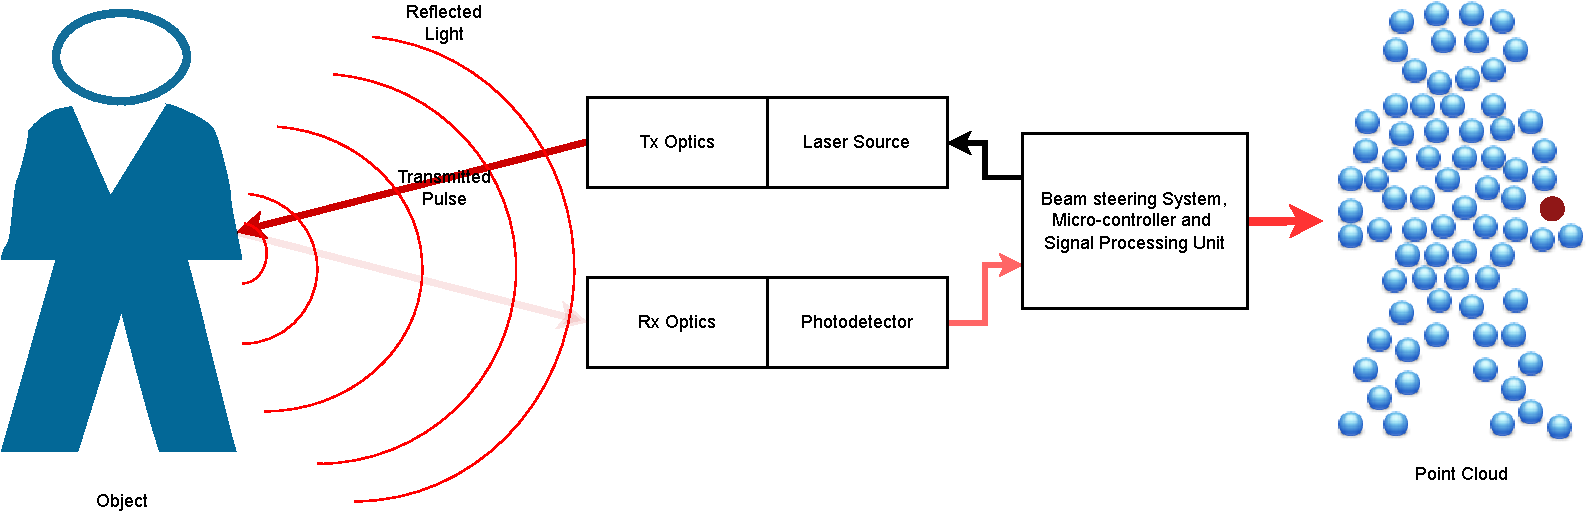
\includegraphics[width=0.8\linewidth]{97_graphics/related_work/lidar_principle.pdf}
    \caption{Operating principle of LiDAR}
    \label{fig:related_work-lidar}
\end{figure}

Laser is an electromagnetic radiation similar to that of radio frequency waves. Lasers are far shorter in wavelength than radio frequency waves, making it simple to use lenses to collimate them into narrow beams. This greatly improves LiDAR's resolution, with less than 2cm accuracy in the case of Velodyne HDL-64E LiDAR \parencite{velodyne_64}, over MIMO imaging radar and reduces the difficulty of estimating the direction of arrival. As shown in figure \ref{fig:related_work-lidar}, laser light is transmitted from the laser source, which is directed by the transmitter optics. The laser ray hits an object, reflecting the laser depending on the properties of the surface. The reflected light is captured by the photodetector system. The time of flight is calculated based on the time between the sending and receiving of the pulse. Based on the time of flight and speed of the light, the range is determined. For a round trip time \(t\), with the velocity of laser light \(c\), the distance \(d\) between the object and the laser source is determined as shown in equation \ref{eq:laser}.
\begin{equation}\label{eq:laser}
    d = \frac{c \cdot t}{2}
\end{equation}
For Speed of light(Approx.) = \(3 * 10^8 m/s^2\) and TOF = \(10 ns = 10 * 10^{-9} second\). We can use equation \ref{eq:laser} to find the distance between the laser source and the target point. Using the formula we get, the distance between the laser source and target = 0.15 meters. So it means that the distance between the laser source and the target hit point is 0.15 meters. By using the orientation of the LiDAR sensor, the exact position of the hit point is calculated. For example, if the LiDAR sensor was oriented along the x-axis, then the coordinate of the hit point would be \((x, y, z) = (0.15, 0, 0)\). Finding each point from the environment gives a point cloud representation of the environment. Data from LiDAR sensors are stored in the form of binaries. The point cloud from the LiDAR can also be represented in formats such as LAS/ LAZ, PLY, ASCII, BIN, text, etc.

\section{Testing Highly Autonomous Driving Systems}
Since autonomous driving systems are getting more complicated, they need to be extensively examined before being released for public use. Safeguarding the passengers' safety within an autonomous driving system presents a formidable challenge. Throughout the whole phases of development, including functional engineering and testing, integration of systems and validation, test drive and validation, etc., a comprehensive profile for testing of autonomous vehicle procedures is critically needed. Figure \ref{fig:related_work-ad_testing} shows pipelines in autonomous driving development and testing.

\begin{figure}[htbp]
    \centering
    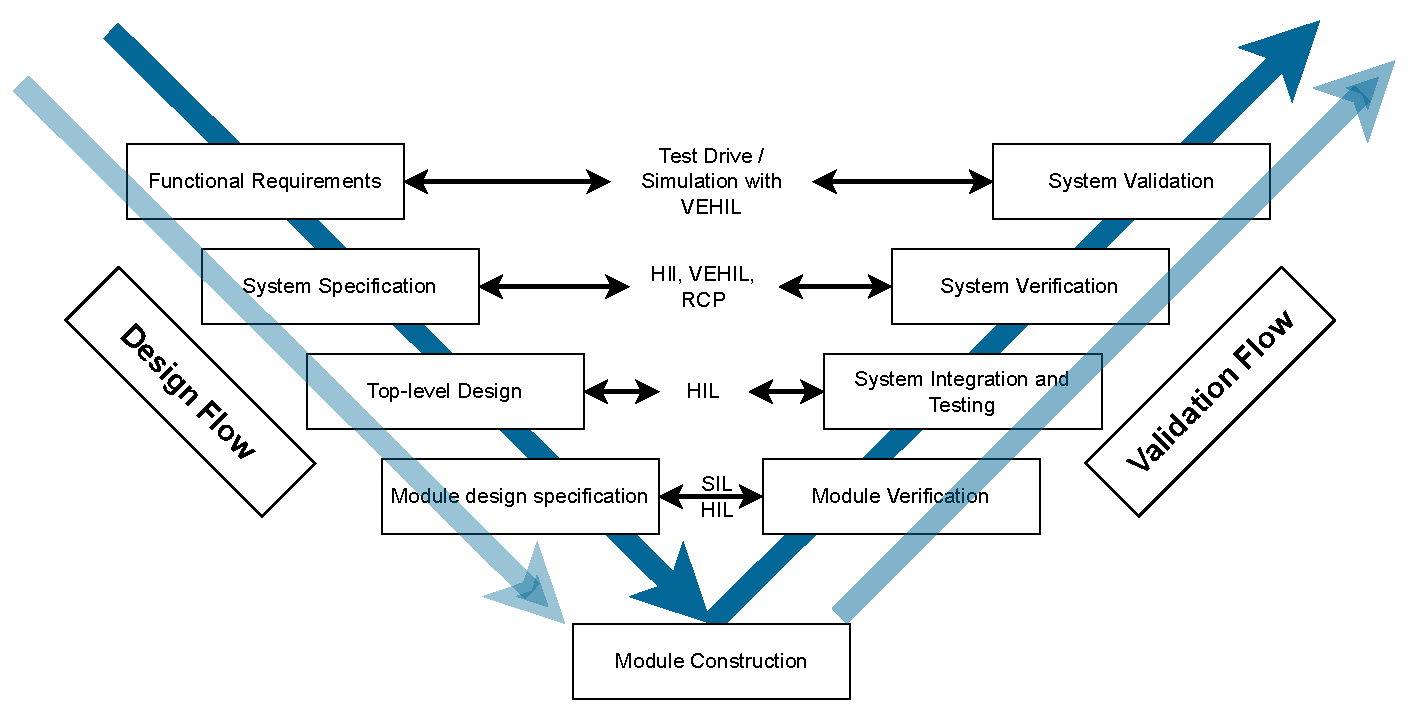
\includegraphics[width=0.7\linewidth]{97_graphics/related_work/ad_testing.pdf}
    \caption{Design and Testing pipeline for Autonomous vehicles, adapted from \parencite{ad_test_2016}}
    \label{fig:related_work-ad_testing}
\end{figure}

Various steps involve from describing functional requirements to development, validation, and verification of the requirement. \acrfull{mil}, \acrfull{sil}, \acrfull{hil}, \acrfull{vil}, or mixed simulation techniques are used to guarantee \acrshort{had} systems functionality, dependability, and safety.  

\begin{figure}[htbp]
    \centering
    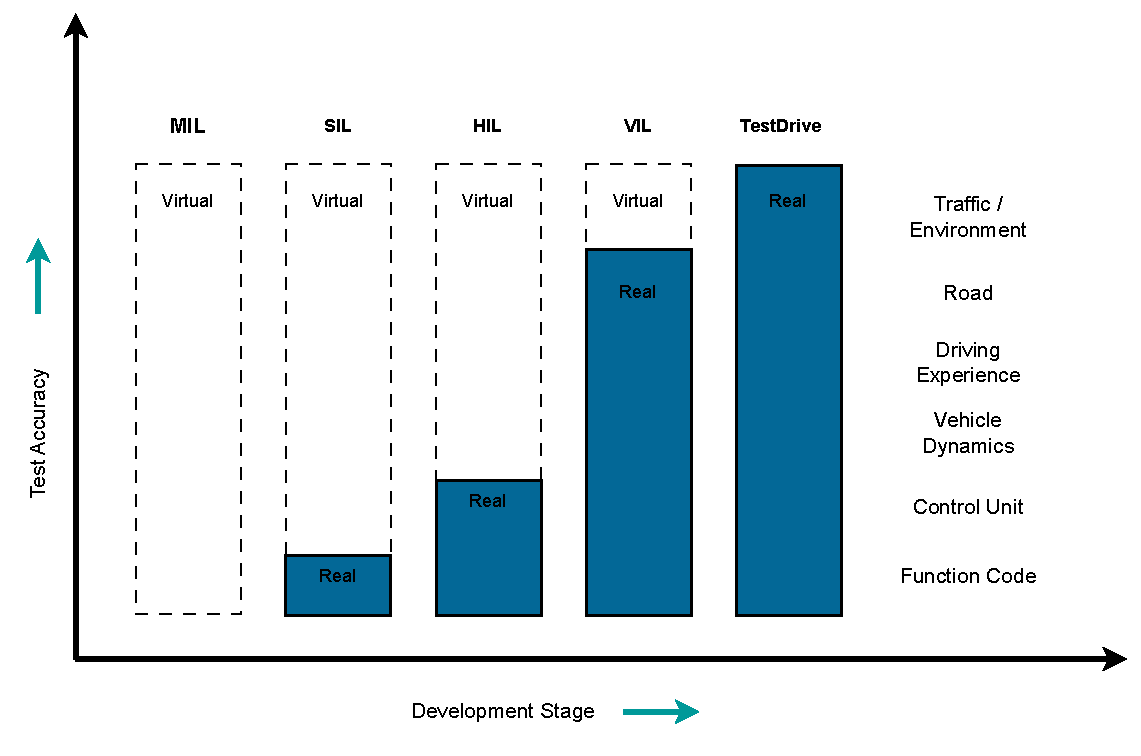
\includegraphics[width=0.7\linewidth]{97_graphics/related_work/x_in_loop_tests.pdf}
    \caption{\acrfull{xil}, adapted from \parencite{x_in_loop_test_compare}}
    \label{fig:related_work-x_in_loop_tests}
\end{figure}

A comparison of various tests concerning their reliability and development lifecycle can be viewed in figure \ref{fig:related_work-x_in_loop_tests}. \acrfull{mil} is a highly helpful tool for rapidly creating and evaluating algorithms during the prototyping or initial test stage. Pseudo code that is ready to be implemented on the \acrshort{had} system needs to be tested. Instead of testing directly on the \acrshort{had} system, which might be hazardous, the \acrfull{sil} approach is carried out. In SIL, only the pseudo-code that is to be implemented in the actual automotive controller in the HAD system is not synthetic, other domains such as \acrfull{ecu}, Vehicle Dynamics, Driving experience, road, traffic, and environment are all implemented in simulations. Numerous situations can be checked quickly because trials can be simulated more quickly than in real life. Hence, MIL and SIL are executed at the initial development phase and also have lower test accuracy in comparison to real-drive testing. Based on environmental data gathered by LiDAR, radar, stereo cameras, and other sensors, the \acrfull{ecu} controller manages the vehicle's supervisory control. With the gathered data, ECU needs to be able to understand the surrounding environment where it acts as a perception unit. It might need to be able to make decisions about safety rules, traffic laws, etc where it supports decision-making. It might also support on sending control signals to the actuators of the HAD system. An HAD system comprises multiple ECUs each focused on specific tasks, and this number only rises when pursuing towards higher level of autonomy in the HAD system. In a lab setting, \acrfull{hil} verifies the real ECU design and operational characteristics at the hardware level. Testing multiple ECUs in a synthetic environment and vehicle makes the development and verification phase of ECUs faster. \acrfull{vil} is the testing of a real vehicle in the real world but with a virtual environment. Traffic around a vehicle in the real world is simulated in VIL. It can be utilized for the evaluation of the HAD system behaviors under various critical situations without the threat of collision or hazards. Test drive comes at the final stage of the development phase. The actual vehicle is tested for the verification of the complete system. The reliability of the HAD system can be emphasized by real drive testing. During real-drive testing, an \acrfull{adas} system can get feedback from the takeover or by the engagement of the driver. This makes the process ever-learning, which improves the reliability factor of the HAD system under various scenarios.


\section{SemanticKITTI Dataset}
It is an extensive dataset based on laser technology to advance semantic segmentation research in the field of autonomous driving. Comprehensive point-wise annotations are available for every sequence in the KITTI Vision Odometry Benchmark dataset \parencite{Geiger2012CVPR}. The public dataset was created by gathering real-world data to meet the rigorous requirements for functional testing and improvement of autonomous driving vehicles. The dataset contains rural roads, residential regions, freeway scenes, and inner-city traffic in Karlsruhe, Germany. For 28 classes; such as person, car, road, and vegetation; point-wise annotation is offered. This is the current state-of-the-art dataset for 3D semantic segmentation. The current SOTA 3D semantic models for autonomous driving can also be viewed at \parencite{papers-with-code}, which are also compared using the SemanticKITTI dataset. About more than 1700 hours \parencite{behley2019semantickitti} was required by a group of annotators to label and verify the labeling of the benchmark dataset. Though collected in a variety of different scenes, it does not contain all the variation of data.

\begin{figure}[htb]
    \centering
    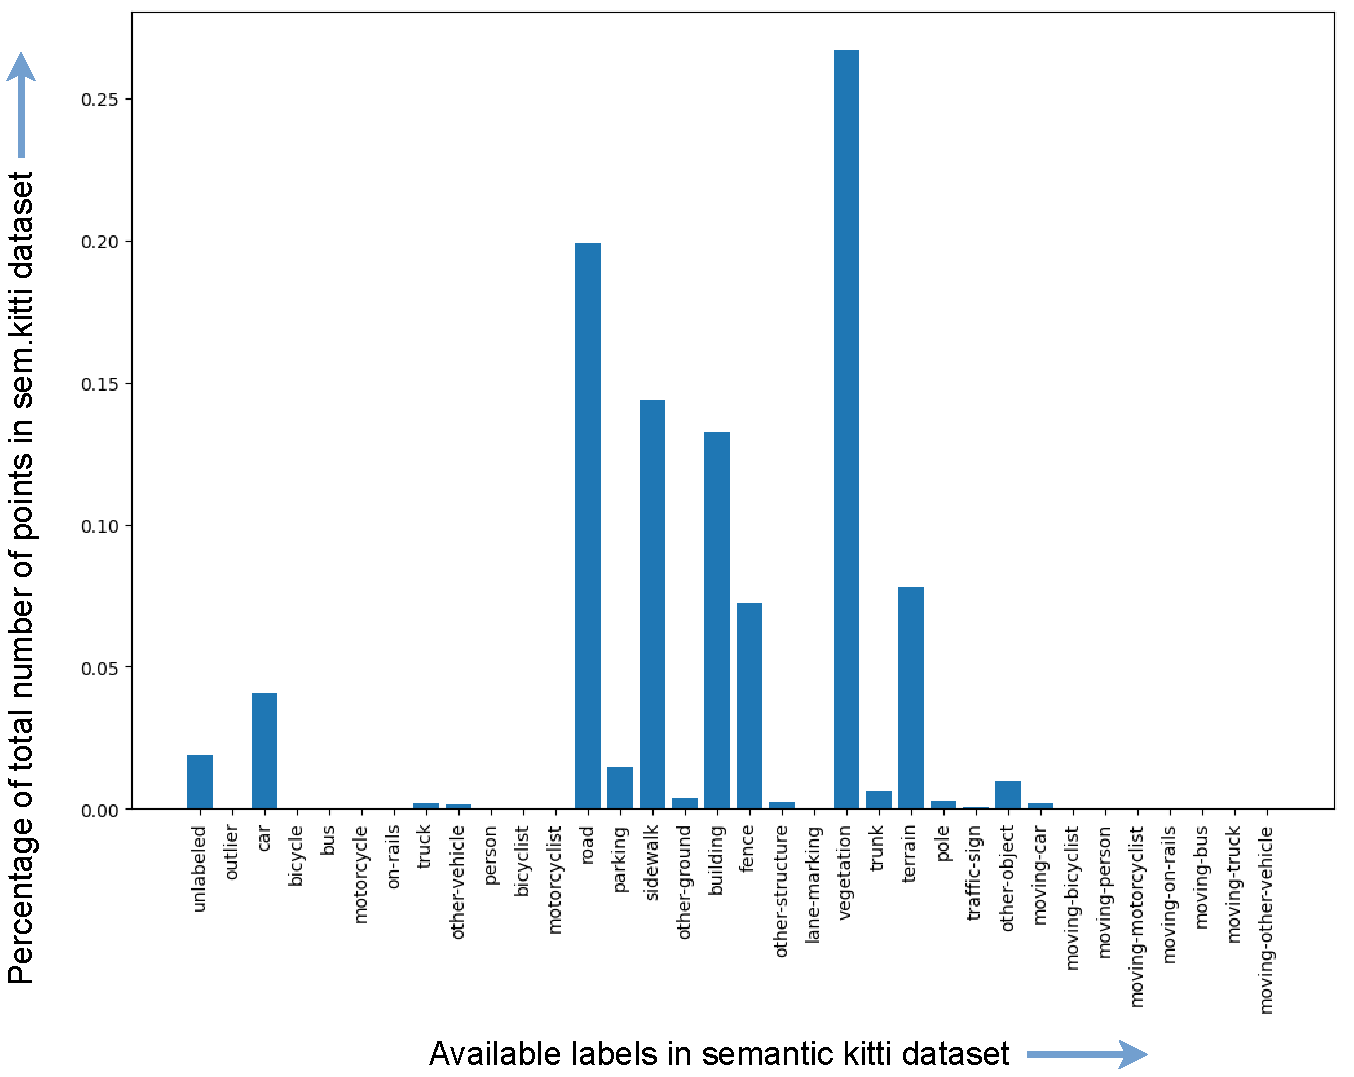
\includegraphics[width=1\linewidth]{97_graphics//related_work/ratio_with_total_points_kitti.pdf}
    \caption{Class distribution in SemanticKITTI Dataset in comparison with complete dataset points}
    \label{fig:related_work-ratio_with_total_points_kitti}
\end{figure}

Figure \ref{fig:related_work-ratio_with_total_points_kitti} shows variants of classes in comparison with total labeled classes available in the SemanticKITTI dataset \parencite{behley2019semantickitti, sem_kitti_total_points_ratio}. From the figure, it can be visualized that vegetation is the most labeled class, after that are roads, sidewalks, buildings, fences, etc. The number of labeled points for classes like person, car, trucks, etc is relatively low in comparison with classes like road, building, fence, vegetation, terrain, etc. The dataset contains scenes with either a higher density of vegetation or scenes of downtowns, as shown in the figure. For a HAD system, any situation can occur when navigating in an environment such as across a river, along a mountain trail, through a desert, alongside an under-construction region, or through a huge mass of people due to demonstration, etc. Such scenarios datasets are not made available in the SemanticKITTI dataset as the data was collected in a controlled setting in Karlsruhe, Germany. This presents a gap in the dataset to represent scenarios to a maximum extent and hence only represent the real world in fragments. Also since the performance of LiDAR is also affected by environmental factors \parencite{park2023automotive}, the dataset is not enough to represent the real world to a maximum extent in the HAD context.

\begin{figure}[htb]
    \centering
    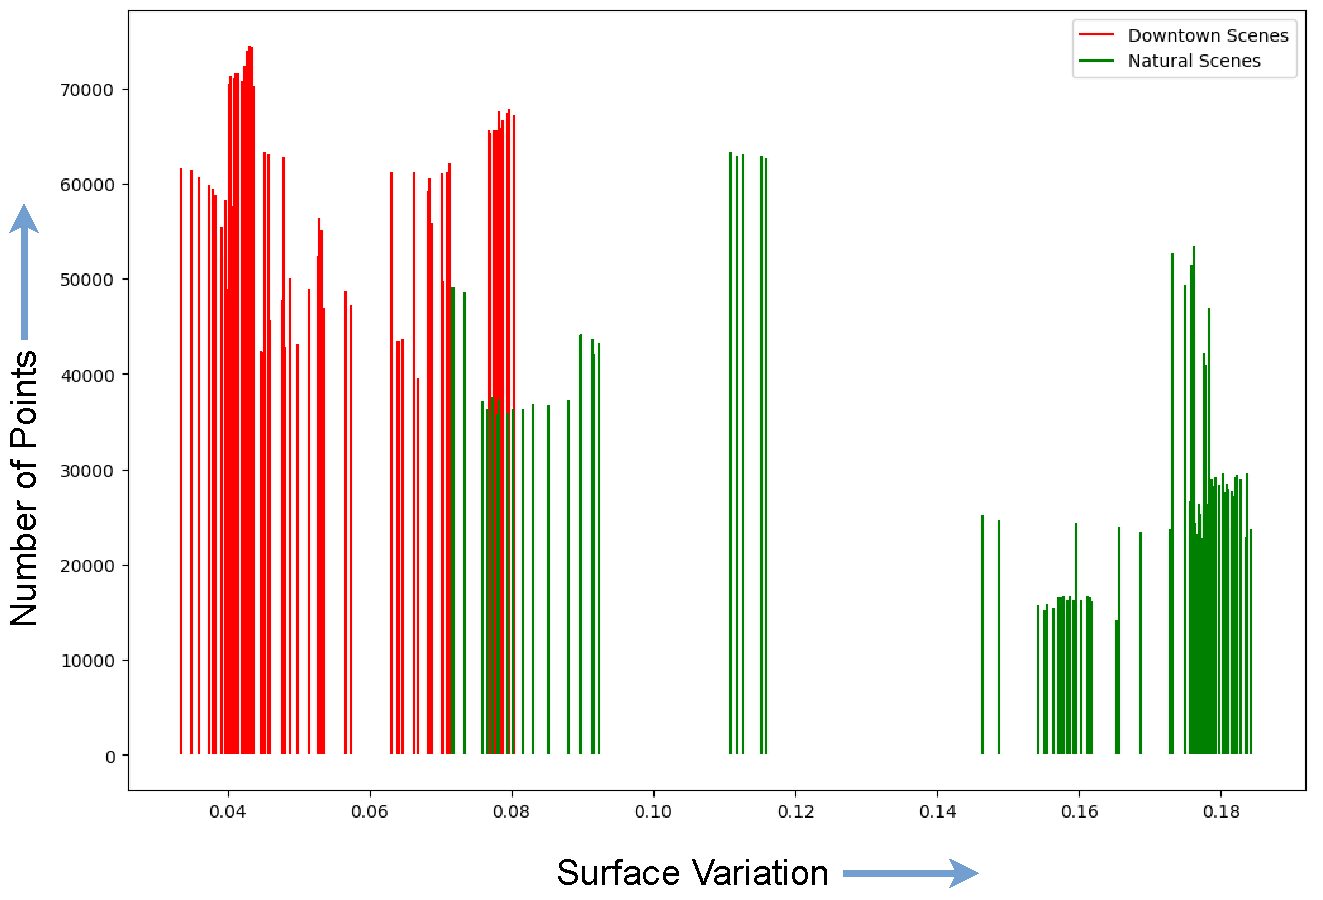
\includegraphics[width=1\linewidth]{97_graphics/related_work/downtown_and_vegetation_sv.pdf}
    \caption{Distribution of SemanticKITTI Datasets}
    \label{fig:related_work-downtown_and_vegetation_sv}
\end{figure}

From a randomly selected 100 LiDAR sequences from the SemanticKITTI dataset, point clouds for downtown were calculated by accumulating points for buildings, fences, vehicles, parking, etc, unlabeled points, outliers, roads, vegetation, trunks, terrain, other-objects points were not taken to be the points for downtown for the calculation in figure \ref{fig:related_work-downtown_and_vegetation_sv}. For the point clouds of vegetation; vegetation, trunk, and terrain point clouds were combined. Point cloud aggregation is performed independently for downtown and vegetation categories within each sequence. Using hybrid search in open3d \parencite{open3d} with a sphere of radius 30 cm and maximum nearest neighbor of 6 for nearest neighbor search, surface variation was calculated using the equation \ref{eq:surf_var}. The average was taken after dividing the sum of the surface variation of each point by the total number of points for a scene for either downtown or vegetation separately. Figure \ref{fig:related_work-downtown_and_vegetation_sv} shows the distribution of geometric features of the dataset for each scene. The red lines represent downtown and the green lines represent vegetation. It can be analyzed that the dataset is not evenly distributed when comparing the geometric features. The available SOTA dataset does not represent diverse scenes and it is risky, expensive, and not usually reproducible to physically test HAD vehicles on public roads. Thus, rather than doing real-world testing, simulations and other methods are opted for the initial testing phase.




\section{Simulations}
Collection of large annotated datasets like SemanticKITTI requires extensive labor work\parencite{behley2019semantickitti}. The situation becomes considerably more problematic when sparse LiDAR data is included. In order to prevent overfitting and enhance neural networks' capacity for generalization by intentionally increasing the number and variety of training data, simulations are used. Simulation are very useful in generating a variety of scenarios which is risky, costly, and rare to get from the real world. However, the variation and unpredictability of real-world situations, such as interactions between automobile drivers, pedestrians, and environmental elements, may not always be adequately captured by simulations.
\begin{figure}[htbp]
    \centering
    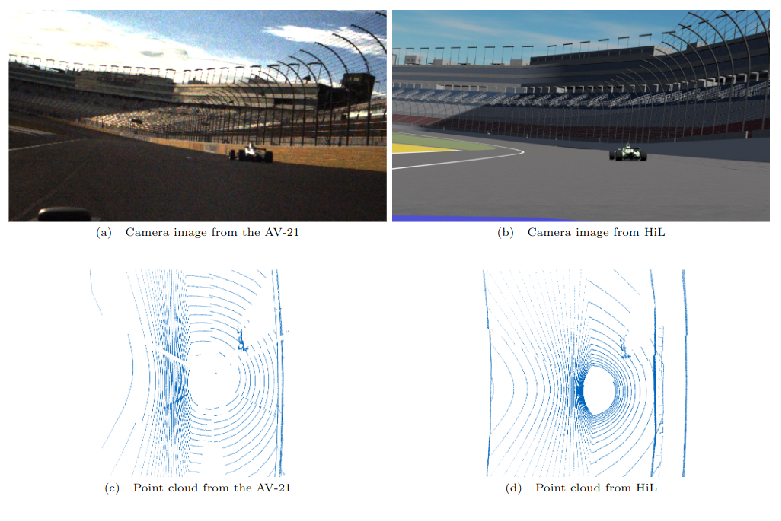
\includegraphics[width=0.8\linewidth]{97_graphics/related_work/real_vs_simulation_difference.pdf}
    \caption{Real world vs Simulation difference \parencite{sauerbeck_learn_Year}}
    \label{fig:related_work-real_vs_simulation}
\end{figure}

Data captured on a series of Indy Autonomous Challenge 2021 \parencite{sauerbeck_learn_Year} shows the difference between the real environment and synthetic simulation. The assumptions that underpin virtual sensor models do not always stand valid in practical situations. Content and Appearance gap between the synthetic and real-world is also discussed in \parencite{care_real_and_syn_gap}. For high accuracy, we need simulation with a low domain gap concerning the real world. It is difficult to model HAD simulators involving LiDAR because of the following reasons \parencite{zero_domain_gap}. 
\begin{itemize}
    \item Unreturned pulses because of pulse's power decay
    \item Multiple echoes from the environment resulting in multiple peaks in the returning signal
    \item Spurious returns due to volume scattering, blooming, beam divergence, multi-echo, etc.
    \item Noisy points because of randomness in the real world, retro-reflectors.
    \item Rolling shutter and motion blur in moving vehicle
\end{itemize}

\section{Scenario-Based Testing}
According to \parencite{def_scene}, a scene is a description of a particular moment in time of the environment that includes the scenery, dynamic aspects, self-representations of all the performers and spectators, and the interactions between those entities. A scenario explains how various scenes in a series of sequences of scenes evolve over time. Three distinct scenarios are defined according to \parencite{menzel2018scenarios}. They are functional scenarios, logical scenarios, and concrete scenarios. 

\begin{figure}[htbp]
    \centering
    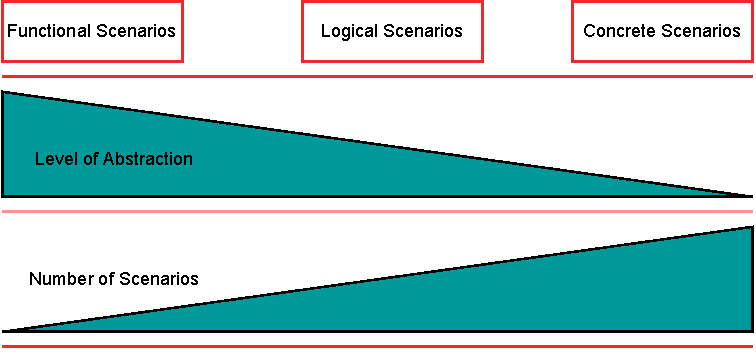
\includegraphics[width=0.75\linewidth]{97_graphics/related_work/three_different_scenarios.pdf}
    \caption{Three different scenarios, adapted from \parencite{menzel2018scenarios}}
    \label{fig:related_work-3scenarios}
\end{figure}

As shown in figure \ref{fig:related_work-3scenarios}, the level of abstraction decreases with an increase in several scenarios from functional to concrete scenarios. Functional scenarios come in the concept phase where the scenarios can be described by human experts in the natural language. A logical scenario appears in the system development phase where the scenario is explained with various parameter ranges. Concrete scenarios are represented for the test phase where the concrete state values are defined to guarantee scene replicability and facilitate testing techniques. For describing the parameters of the logical and concrete scenario, a five-layer model is explained in \parencite{bagschik2018ontology}, as shown in figure \ref{fig:related_work-5layer_model}.

\begin{figure}[htbp]
    \centering
    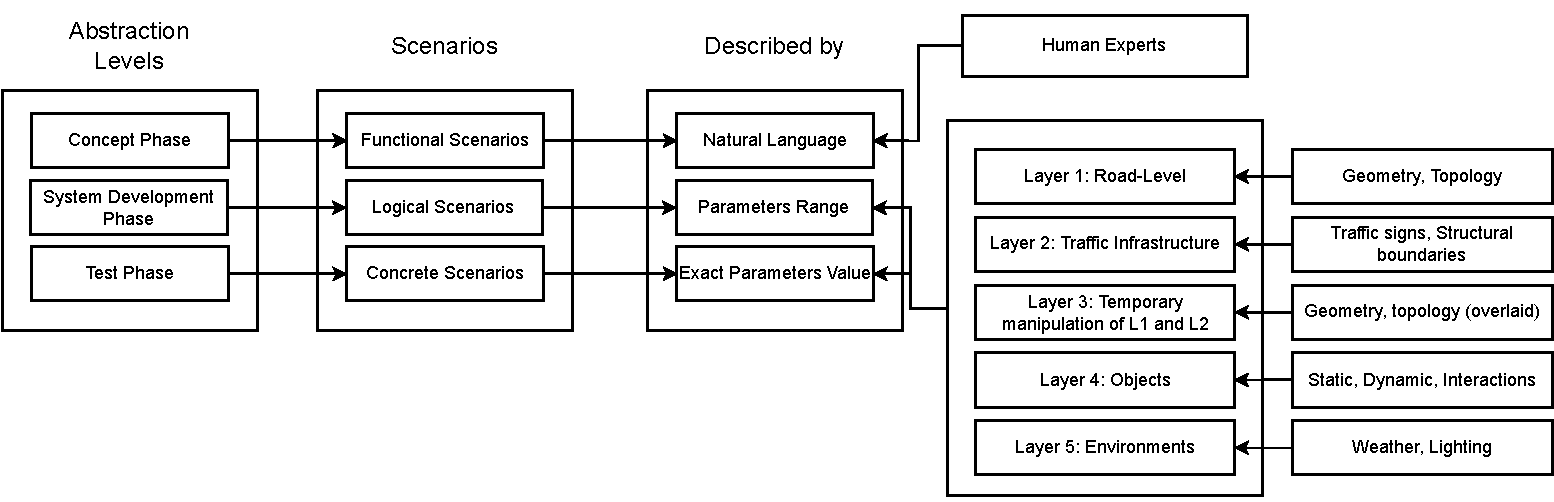
\includegraphics[width=1\linewidth]{97_graphics/related_work/scenario_based_testing.pdf}
    \caption{Abstraction levels, scenarios, and explanation terms. Adapted from \parencite{bagschik2018ontology} and \parencite{menzel2018scenarios}
    }
    \label{fig:related_work-5layer_model}
\end{figure}

To arrange all the data in a database of knowledge to represent scenes, a model with multiple layers is explained as illustrated in the figure \ref{fig:related_work-5layer_model}. The topology and markings of the road are described in the first layer. The model's hierarchical ideas describe how to construct legitimate road fragments for traffic scenes by assembling geometries that represent lanes. Road-level traffic infrastructure is added in the second layer. Not every stationary object, such as vegetation, is a part of the infrastructure for traffic. Classes that reflect the marking, routing, and security requirements for building sites are included in the third layer. In the ensuing traffic scenarios, the modifications made to the original layout are identified as manipulation. The fourth layer models every object that may not be included in the transportation infrastructure. It is possible to arrange both stationary and mobile objects without significantly altering the connections within the traffic infrastructure. Participants in traffic are divided into object classes, such as vehicles, trucks, bicycles, etc. Environmental conditions like weather and lightning are considered on the fifth layer. Additionally, the impact on the interactions amongst traffic participants is taken into account, leading to varying parameter ranges for relative parameters.

With the help of the scenarios database and knowledge, new scenarios are generated. The information content and level of abstraction in each generated or extracted scenario categorize the scenario types. The scenarios database is created with expert knowledge or by varying the parameter range and values. As described on \parencite{bagschik2018ontology}, concrete scenarios are selected based on a testing-based approach or falsification-based approach. In the testing-based approach, range sampling and distribution sampling are done from a logical scenario database, and concrete scenarios are extracted. Based on macroscopic and microscopic assessment, a scenario is selected. A substantial quantity of data needs to be made available to make a macroscopic (statistical) assessment regarding the overall effect of autonomous vehicles on traffic. Specific traffic scenarios are put to the test and assessed. Microscopic evaluation is the assessment of a single scenario. The purpose of the falsification techniques is to locate counterexamples that break safety regulations while doing microscopic evaluations. Based on criticality, complexity, etc concrete scenarios are selected from the scenario database which undergoes microscopic assessment. Scenarios could be samples from the accident database or by changing the criticality of available concrete scenarios. Increasing the scenario's complexity can likewise raise the likelihood of discovering a counterexample.
The chosen specific scenarios can be executed in a variety of testing environments. These can be carried out using \acrfull{xil} simulation \parencite{x_in_loop}, which offers a higher level of virtualization, or in the actual world through field or proving-ground experiments. Since XIL offers numerous benefits in terms of, for example, expenses, risks, and safety, nearly all references employ simulation as part of their proof of concept.

\section{Enhancing Methods for Testing LiDAR-based Functions}
The various methods used to improve the testing of LiDAR functions are described in below steps :
\begin{itemize}
    \item \textbf{Real-world Testing : }
    Testing in real-world settings enables evaluation of LiDAR performance in real-world scenarios, encompassing diverse weather, illumination, and topography conditions.  However, this methodology is risky, uneconomical, and difficult to reproduce in certain conditions. This makes researchers explore the simulators and synthetic data.
    \item \textbf{Simulations and Modeling : }
    Virtual environments that mimic different settings and scenarios make it possible to test LiDAR systems thoroughly without requiring actual setups.  To better understand and forecast sensor performance, physics-based models simulating LiDAR sensor behavior in various environments are utilized.
    \item \textbf{LiDAR Data Augmentation : }
    Capturing data representing diversities of scenes in the real world is expensive and laborious. Simulations are also utilized in addition but because of the domain gap between the real and synthetic world, the captured data do not accurately represent the real world environment. LiDAR data augmentation could be approached where data within the LiDAR is changed like scaled, transformed, rotated, etc. Combining synthetic data of objects with real-world point clouds is also an option.
    \item \textbf{Sensor Data Fusion : }
    The system's reliability is increased by integrating LiDAR data with information from other sensors, including cameras, radar, and \acrshort{gps}, which also improves perception accuracy and redundancy.
    \item \textbf{Benchmarking and Standarization : }
    It is easier to compare various systems and quantify advancements over time when defined criteria and benchmarks are established for analyzing LiDAR performance. Uniformity and dependability across various systems and manufacturers are ensured by adhering to industry standards and guidelines for LiDAR testing.
    \item \textbf{Security testing and Attack Simulations : }
    Testing LiDAR systems for possible security risks like jamming or spoofing guarantees their robustness and resilience when used in real-world scenarios.  Adversarial scenario simulation is used to evaluate LiDAR performance under several attack vectors, which aids in finding weaknesses and strengthening system defenses.
\end{itemize}

\section{Statistical Computation of LiDAR Point Cloud Descriptors}
\subsection{Mathematical Operations in 3D Space}
\subsubsection{Scalars and Vectors}
A scalar is a quantity that has only magnitude or size without any associated direction. Scalars are often employed to quantify quantities like mass, temperature, energy, speed, or time since they are represented by a single real integer. A quantity having both magnitude and direction is called a vector. An ordered collection of real numbers, or components, and a direction in space are used to represent vectors. Vectors are commonly depicted in 3D space as arrows that point from the origin to a designated location in the space.


\begin{figure}[htbp]
    \centering
    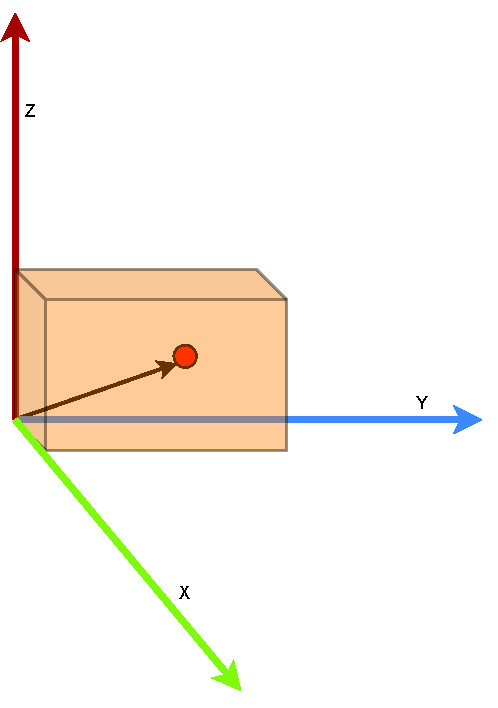
\includegraphics[width=0.4\linewidth]{97_graphics/related_work/scalar_and_vector.pdf}
    \caption{A 3D Cube in XYZ Coordinate System.}
    \label{fig:related_work-scalar_and_vector}
\end{figure}

In the figure \ref{fig:related_work-scalar_and_vector}, the volume of the cuboid represents the scalar quantity, and the black arrow pointing to a red point in the cuboid represents a vector. Scalars can be added, subtracted, multiplied, or divided just like ordinary numbers. Various mathematical operations can be performed on vectors like scalar multiplication, vector addition, dot product, cross product, etc. Equation \ref{eq:dot_product}, \ref{eq:cosine_angle}, \ref{eq:cross_product}, \ref{eq:sine_angle}, \ref{eq:angle_between_vectors} gives a general idea of calculating the angle between two vectors using the vector operations.
\begin{itemize}
    \item \textbf{Dot Product}:
    \begin{equation}\label{eq:dot_product}
        \mathbf{p} \cdot \mathbf{q} = p_x \cdot q_x + p_y \cdot q_y + p_z \cdot q_z
    \end{equation}
    \item \textbf{Cosine of Angle between two vectors}:
    \begin{equation}\label{eq:cosine_angle}
        \cos\theta = \left(\frac{\mathbf{p} \cdot \mathbf{q}}{|\mathbf{p}| \cdot |\mathbf{q}|}\right)
    \end{equation}
    \item \textbf{Cross Product}:
    \begin{equation}\label{eq:cross_product}
        \mathbf{p} \times \mathbf{q} = (p_y q_z - p_z q_y, p_z q_x - p_x q_z, p_x q_y - p_y q_x)
    \end{equation}
    \item \textbf{Sine of Angle between two vectors}:
    \begin{equation}\label{eq:sine_angle}
        \sin\theta = \left(\frac{|\mathbf{p} \times \mathbf{q}|}{|\mathbf{p}| \cdot |\mathbf{q}|}\right)
    \end{equation}
    \item \textbf{Angle between two vectors}:
    \begin{equation}\label{eq:angle_between_vectors}
        \theta = \arctan\left(\frac{\sin(\theta)}{\cos(\theta)}\right)
    \end{equation}
\end{itemize}

\subsubsection{Translation, Rotation, and Transformation}
Moving an object from one place to another in three dimensions without modifying its shape or orientation is referred to as translation. It entails moving every point on the item in a certain direction by a predetermined amount. In three-dimensional space, rotation is the process of shifting an object's orientation around a designated axis or point. It involves rotating the object by a certain angle about the selected axis or point. A combination of translation, rotation, scaling, and other operations performed on an object is referred to as transformation in 3D space. It enables one-step changes to the object's size, location, and orientation. The operations are represented by the equation \ref{eq:translation}, \ref{eq:rotation}, \ref{eq:transformation}. Where (x,y,z) represents a point in cylindrical coordinates and T represents any transformation matrix.

\begin{itemize}
    \item \textbf{Translation}:
    \begin{equation}\label{eq:translation}
        \begin{pmatrix}
        x' \\
        y' \\
        z'
        \end{pmatrix}
        =
        \begin{pmatrix}
        x + a \\
        y + b \\
        z + c
        \end{pmatrix}
    \end{equation}
    
    \item \textbf{Rotation}:
    \begin{equation}\label{eq:rotation}
        \begin{pmatrix}
        x' \\
        y' \\
        z'
        \end{pmatrix}
        =
        \begin{bmatrix}
        \cos(\theta) & -\sin(\theta) & 0 \\
        \sin(\theta) & \cos(\theta) & 0 \\
        0 & 0 & 1
        \end{bmatrix}
        \begin{pmatrix}
        x \\
        y \\
        z
        \end{pmatrix}
    \end{equation}
    
    \item \textbf{Transformation}:
    \begin{equation}\label{eq:transformation}
        \begin{pmatrix}
        x' \\
        y' \\
        z'
        \end{pmatrix}
        =
        T
        \begin{pmatrix}
        x \\
        y \\
        z
        \end{pmatrix}
    \end{equation}
\end{itemize}

\subsection{Nearest Neighbour Search}
A basic issue in mathematics and computer science, especially in the areas of computational geometry and data structures, is nearest neighbor search. A collection of points P serves as the problem's input. The objective is to locate the point in the set P that is closest to a given query point, q. This necessitates O(n) comparisons naively since we must compare q to every point in P. Using the brute-force technique is not computationally possible when the number of points is very huge. As a result, our objective is to pre-process the input and produce a data structure that can respond to queries rapidly. Distance metric, such as the Minkowski, Manhattan, or Euclidean distances, is usually utilized to determine the separation between two positions, which can be used to create new data structures for effective search. The Euclidean distance, which is the square root of the total squared differences in each coordinate, is frequently used in the context of three-dimensional space. Nearest Neighbor has countless applications and is used in numerous computer science fields, including computational linguistics, machine learning, and image recognition. It's crucial to remember that, despite all recent developments in the field, exhaustive search remains the only technique that can reliably retrieve the precise nearest neighbor. Because of the "curse of dimensionality", finding the exact nearest neighbor is impractical when the dimensionality of the data is large and so an Approximate Nearest Neighbor was introduced. Techniques like Vector Transformation, Vector Encoding, None Exhaustive Search Components were introduced to preprocess the data into an efficient index. Numerous space-partitioning techniques have been created to address the nearest neighbor search issue. The k-d tree (a binary tree), which repeatedly splits the search space into two areas with half of the points of the parent region, is arguably the most straightforward. By analyzing the query point at each split, queries are executed by traversing the tree from the root to a leaf. It might also be necessary to assess nearby branches that could contain hits, depending on the query's distance specification. Parameters, such as radius and maximum number of nearest neighbors, could be adjusted for a search of the nearest neighbor of a query point.
\begin{figure}[htbp]
    \centering
    \begin{minipage}[b]{0.45\textwidth}
    \centering
    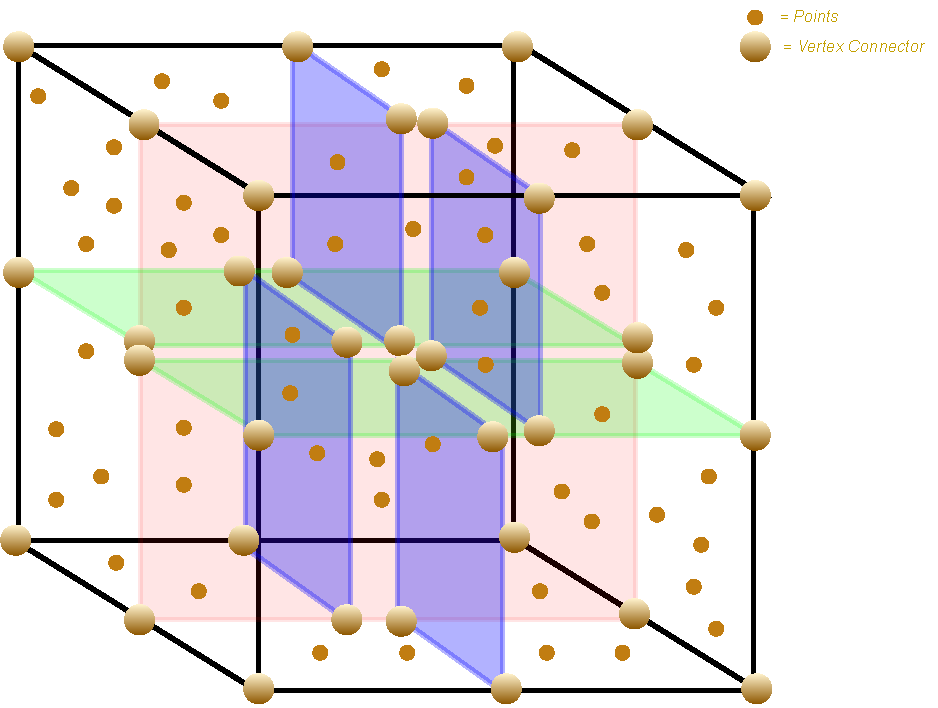
\includegraphics[width=1\linewidth]{97_graphics/related_work/kdtree_cube.pdf}
    \caption{3D Space containing Points with dividing Hyperplanes.}
    \label{fig:related_work-kdtree}
    \end{minipage}
    \hfill
    \begin{minipage}[b]{0.45\textwidth}
    \centering
    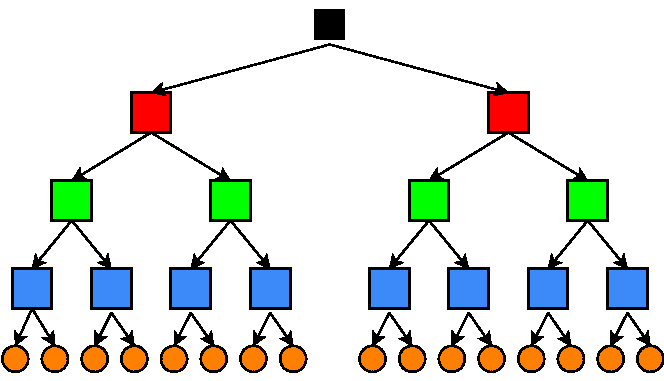
\includegraphics[width=1\linewidth]{97_graphics/related_work/kdtree_tree.pdf}
    \caption{Tree structure showing leaf nodes, root nodes.}
    \label{fig:related_work-search_tree}
    \end{minipage}
\end{figure}

In figure \ref{fig:related_work-kdtree}, the initial partition (the red vertical plane) divides the root cell into two subcells. The subsequent division (the green horizontal planes) further divides each of those subcells into two subcells, and so on. The splitting plane in the three-dimensional space represents the non-leaf node. All non-leaf nodes can be viewed as inherently creating a dividing hyperplane, or half-space, that divides the available region into two halves. Points to the left of the hyperplane are represented by the subtree on the left side of that node, while points to the right of the hyperplane are represented by the subtree on the right side. Here's how to figure out the orientation of the hyperplane: each node in the tree corresponds to one of the k dimensions, and the hyperplane is oriented perpendicularly to the axis of that dimension. This splitting of 3D dimension into cells can be discussed with the figure \ref{fig:related_work-search_tree}. The square boxes in the figure represent non-leaf nodes. The circular shapes in orange color represent the points in the 3D space. A 3D space is split into two halves by a red plane in figure \ref{fig:related_work-kdtree}. This is represented by the back root node separated into two red-colored child nodes - left and right node. The red plane is further divided into two green planes in the 3D space, which is represented by two green-colored child nodes of red parent nodes. The space separated by green planes is further divided by blue planes, which contain the points. A search of the nearest neighbor is done by traversing the tree from the root to the leaf nodes, where each comparison is done for each dimension of k-dimensions alternatively when traversing the parent nodes.

\subsection{Variance, Covariance, and Covariance Matrix}
The dispersion or spread of a single random variable is measured by variance. The variance of X in 3D space expresses the degree to which the values of X differ from their mean value. The amount that two random variables fluctuate together is measured by covariance. 

\begin{itemize}
    \item \textbf{Variance of variable X:}
    \begin{equation}
    \text{Var}(X) = \frac{1}{n} \sum_{i=1}^{n} (X_i - \bar{X})^2
    \end{equation}
    
    \item \textbf{Covariance between X and Y:}
    \begin{equation}\label{eq:covariance}
    \text{Cov}(X, Y) = \frac{1}{n} \sum_{i=1}^{n} (X_i - \bar{X})(Y_i - \bar{Y})
    \end{equation}
    
    \item \textbf{Covariance Matrix in 3D Spaces:}
    The covariance matrix \(C\) is given by:
    \begin{equation}\label{eq:covariance_matrix}
    C = \begin{bmatrix}
    \text{Var}(X) & \text{Cov}(X, Y) & \text{Cov}(X, Z) \\
    \text{Cov}(Y, X) & \text{Var}(Y) & \text{Cov}(Y, Z) \\
    \text{Cov}(Z, X) & \text{Cov}(Z, Y) & \text{Var}(Z)
    \end{bmatrix}
    \end{equation}
\end{itemize}

The equation \ref{eq:covariance_matrix} is very useful in giving us insights about the dataset of variables by helping us to understand the relation between variables, in our case in 3D space. It can be summarized in below points :
\begin{itemize}
    \item  Negative covariances show that variables move in the opposite way.
    \item Positive covariances show that variables tend to rise or decrease together.
\end{itemize}

It can be utilized to construct a transformation matrix known as a whitening transformation, which, from another angle, enables one to evaluate the best foundation for compactly describing the data or, alternatively, to fully decorrelate the data. Therefore, the covariance matrix can be viewed as a linear transformation that maps vectors from one d-dimensional space to another d-dimensional space. Dimensionality Reduction, financial portfolio optimizations, clustering, statistical inference, and calculation of surface orientations are some use cases from the use of covariance matrix.

\subsection{Eigen Values and Eigen Vectors}
 The vectors that a linear transformation works on are rotated, stretched, or sheared. The vectors that are merely stretched; they do not rotate or shear; are known as its eigenvectors. The associated eigenvalue for an eigenvector is the value that influences an eigenvector to change in length or direction. If the eigenvalue is negative, the eigenvector's direction is transformed. Non-zero vectors that, upon application of a linear transformation (expressed by a matrix), are scaled by the associated eigenvalues are Eigenvectors. Eigenvectors depict the directions that a transformation acts in, just extending or compressing; they do not alter the direction. For a transformation matrix "T", the corresponding eigen values and eigen vectors are represented by equation \ref{eq:eigen}. If \( \lambda_1, \lambda_2, \) and \( \lambda_3 \) represents the eigen values of a 3D covariance matrix then a relation can be showed by equation \ref{eq:eigen_relation}.

\begin{itemize}
    \item Eigenvalue (\( \lambda \)) and Eigenvector (\( \mathbf{v}^{\rightarrow} \)):
    \begin{equation}\label{eq:eigen}
    \text T \mathbf{v}^{\rightarrow} = \lambda \mathbf{v}^{\rightarrow}
    \end{equation}
    \item Relation between eigen values for a 3D Covaraiance matrix :
    \begin{equation}\label{eq:eigen_relation}
    \lambda_1 \geq \lambda_2 \geq \lambda_3 \geq 0
    \end{equation}
    
\end{itemize}

By undergoing the process of eigen decomposition using the equation \ref{eq:eigen}, eigen vectors and eigen values can be calculated from the covariance matrix. Principal components analysis makes use of eigenvectors and eigenvalues, where eigenvectors are associated with the principal components, and eigenvalues explain the discrepancies of the principal components. Some Key features can be described as :
\begin{itemize}
    \item High value of eigenvector captures directions of maximum variance of data.
    \item Low value of eigenvector captures directions of minimum variance of data.
    \item Sum of eigenvalues gives the total variation of points from the center of gravity.
    \item For n-dimensional data, at most n eigenvalues and corresponding eigenvectors is possible
\end{itemize}

Selecting a subset of the eigenvectors that represent the maximum variance of data allows for dimensionality reduction while preserving the most important features. It is used in applications like normal calculation, feature extraction, vibration analysis, etc.

\subsection{Normal Estimation}
In computer vision, computer graphics, and geometric modeling, normal estimation is an essential procedure. To accurately recreate the underlying surface geometry, surface reconstruction techniques frequently begin with normal estimation, which involves determining the normals of a point cloud or a group of surface points. When working with scarce or noisy data, normal information helps create surfaces that are accurate and smooth. Normals aid in the identification of sharp edges, the determination of surface features, and the direction of different mesh processing activities. Rendering scenes with accurate normal estimates makes them look more realistic. For robots to navigate challenging environments and interact with items effectively, accurate normal information is necessary.

\begin{figure}[htbp]
    \centering
    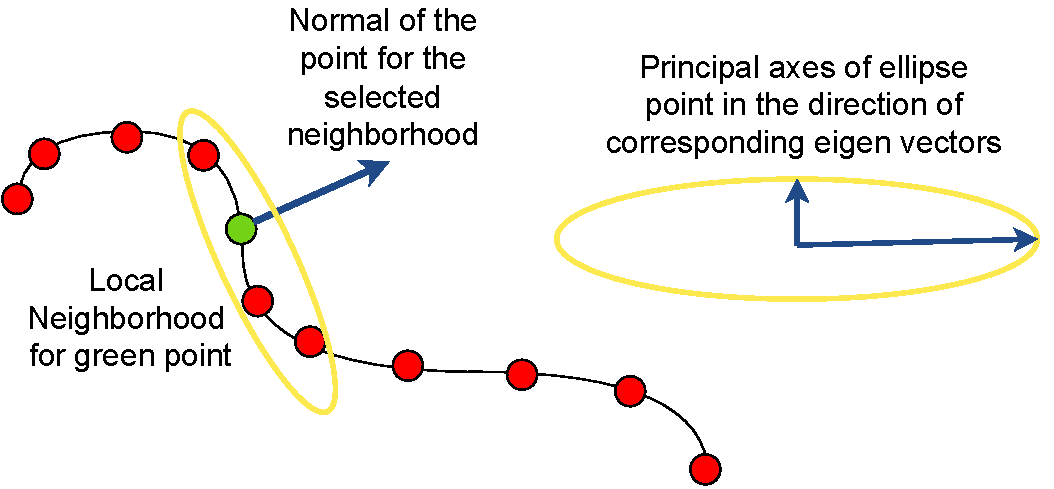
\includegraphics[width=0.5\linewidth]{97_graphics//related_work/normal_estimation.pdf}
    \caption{Surface represented by points and selection of local neighborhood, adapted from \parencite{normal_estimation}}
    \label{fig:related_work-normal_estimation}
\end{figure}

In figure \ref{fig:related_work-normal_estimation}, the black curve represents a surface represented by a group of red points. The orientation of the surface in the region bounded by the yellow color curve represents the normal of the surface for the yellow-bounded region, this is represented by the direction of the blue arrow. We can find the normal of the surface at a point by the following steps \parencite{normal_estimation} referencing the figure \ref{fig:related_work-normal_estimation} :

\begin{enumerate}
    \item Identify the neighbors for the point (represented by a green-colored point in the figure) through which the normal is to be calculated. The neighborhood is represented by the yellow ellipse. 
    \item Calculation of Covariance Matrix from the local neighborhood.
    \item Calculation of Eigen Values and Eigen Matrix by Eigen decomposition of Covariance Matrix.
    \item The Direction of the eigenvector corresponding to the least eigenvalue is the surface normal. (i.e. direction of least variance of the features)
\end{enumerate}

\subsection{Statistical Point Cloud Measurement}
The spatial placement of individual 3D points implicitly represents important geometric information found in 3D point clouds. These attributes should be calculated with particular spatial support because context is not taken into account when considering individual points \parencite{weinmann2013feature}. Usually, the local neighborhood surrounding each 3D point is retrieved in order to explain this implicit information sufficiently. For example, defining a fixed size sphere around a point in a point cloud could give a local neighborhood where all the points lying in the sphere are the neighbors \parencite{lee2002perceptual}. The local 3D structure can be described directly by the eigenvalues of a 3D covariance matrix which follows the equation \ref{eq:eigen}. Alternatively, additional measures that capture unique geometric features can be deduced based on these eigenvalues. The definition of various features are referenced \parencite{weinmann2013feature}.

\begin{itemize}
    \item Linearity (\( L_{\lambda} \)):
    \begin{equation}
        L_{\lambda} = \frac{\lambda_1 - \lambda_2}{\lambda_1}
    \end{equation}
    
    \item Planarity (\( P_{\lambda} \)):
    \begin{equation}
        P_{\lambda} = \frac{\lambda_2 - \lambda_3}{\lambda_1}
    \end{equation}
    
    \item Scatter or Sphericity (\( S_{\lambda} \)):
    \begin{equation}
        S_{\lambda} = \frac{\lambda_3}{\lambda_1}
    \end{equation}
    
    \item Omnivariance (\( O_{\lambda} \)):
    \begin{equation}
        O_{\lambda} = \left( \lambda_1 \cdot \lambda_2 \cdot \lambda_3 \right)^{\frac{1}{3}}
    \end{equation}
    
    \item Anisotropy (\( A_{\lambda} \)):
    \begin{equation}
        A_{\lambda} = \frac{\lambda_1 - \lambda_3}{\lambda_1}
    \end{equation}
    
    \item Surface Variation \parencite{rusu2009semantic} (\( C_{\lambda} \)):
    \begin{equation}\label{eq:surf_var}
        C_{\lambda} = \frac{\lambda_3}{\lambda_1 + \lambda_2 + \lambda_3}
    \end{equation}
    
\end{itemize}

\begin{figure}[htbp]
    \centering
    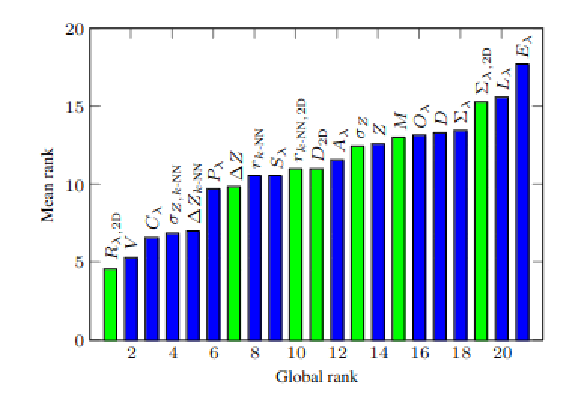
\includegraphics[width=0.6\linewidth]{97_graphics/related_work/geometric_features_ranking.pdf}
    \caption{Mean ranking of the derived features - 3D by blue and 2D by green \parencite{weinmann2013feature}}
    \label{fig:realted_work-3dgeo_feature_assessment}
\end{figure}

Various measures like F-score, Gini Index, Information Gain, Pearson correlation coefficient, and ReliefF were considered from the training data for the ranking of features. From the features ranking as shown in figure \ref{fig:realted_work-3dgeo_feature_assessment}, \( R_{\lambda,2D} \), V and \(C_{\lambda} \) are the most prominent features. \( R_{\lambda,2D} \) is a robust feature for detecting the exterior of the building, the verticality V is a promising feature in differentiating facades from the ground, and \(C_{\lambda} \) is a powerful feature in understanding the difference between planar and non-planar structures \parencite{weinmann2013feature}. Among the prominent features, an in-depth review of surface variation is explained.

\subsubsection{Surface Variation}

\begin{figure}[htbp]
    \centering
    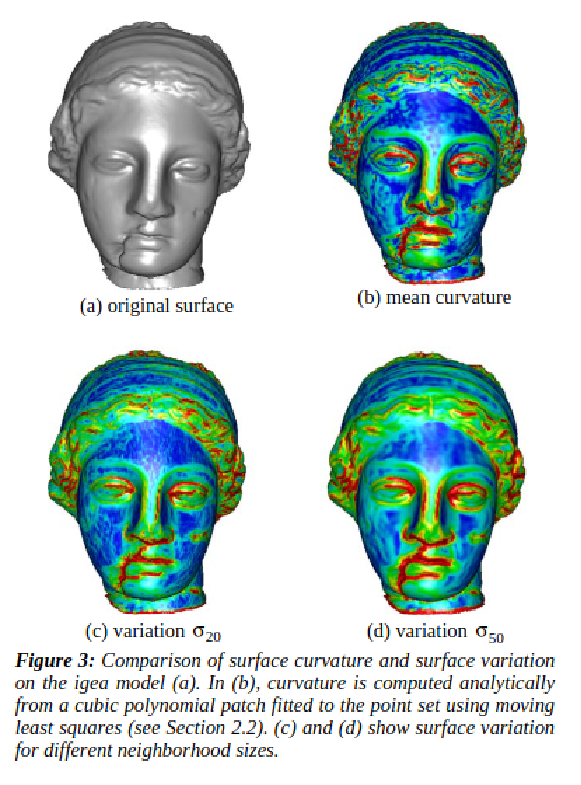
\includegraphics[width=0.6\linewidth]{97_graphics/related_work/surf_variation_with_description.pdf}
    \caption{Visualization of Surface Variation, referenced from \parencite{pauly2002efficient}}
    \label{fig:related_work-surface_variation_visualize}
\end{figure}

As shown in equation \ref{eq:surf_var}, surface variation, also known as surface roughness or surface irregularity, is the ratio between the minimum eigenvalue and the sum of eigenvalues. The surface variation of a point centered in a local neighborhood gives the change in curvature. This feature is invariant to scaling. A smaller value of the surface variation for that point indicates that all points in the local neighborhood lie on a tangential plane to the surface. The value of the surface variation of a point is dependent on the selected neighborhood. The selected neighboring point influences the covariance matrix, which influences the eigenvalues and hence the surface variation is varied. If \(C_{\lambda} = 0 \), then all the points of the neighborhood are located in the plane. \(C_{\lambda} = \frac{1}{3} \) is considered to be the value of isotropically distributed points \parencite{pauly2002efficient}. Figure \ref{fig:related_work-surface_variation_visualize} shows the variation of features for an igea model. Various applications are possible by the analysis of surface variation such as quality control in manufacturing, surface reconstruction, designing components, etc.

\section{Surface Reconstruction}
The process of turning a collection of discrete points or a point cloud into a digital representation of an uninterrupted surface is known as surface reconstruction. It is essential in computer vision, computer graphics, and geometric modeling because it makes it possible to create 3D models from the real-world data that is acquired by sensors like depth cameras, LiDAR scanners, or other photogrammetry methods. Among various available methods for surface reconstruction, three are discussed.

\subsection{Alpha Shapes}
Alpha shape as explained in \parencite{edelsbrunner1983shape}, is the generalization of a convex hull. As clarified on \parencite{alpha_shapes_stanford}, \(\alpha-shape\) can be described as follows. Envision a massive ice cream mass forming a region, with the "hard" chocolate chunks represented as points on the region. All the areas of the ice cream mass are carved out that can be reached without running into pieces of chocolate by using ice cream spoons shaped in the form of a sphere. As a result, we even create holes inside the block (i.e., portions that are not accessible by just sliding the spoon from the outside). Eventually, what we have will be an object surrounded by caps, arcs, and points, but not necessarily convex.  The \(\alpha-shape\) of the points(chocolate toppings) could be understood by adjusting all the  "round" faces into triangles and line segments. \(\alpha\) in \(\alpha-shape\) represents the radius of the carving spoon, which determines the level of detail of the constructed surface. A higher value of alpha results in larger and simpler shapes with lower details. A lower value of alpha results in shapes with finer details. In figure \ref{fig:related_work-alpha_shapes}, points represent chocolate toppings and circles represent spherical ice-cream spoons in 2D space.

\begin{figure}[htbp]
    \centering
    \begin{minipage}[b]{0.45\textwidth}
    \centering
    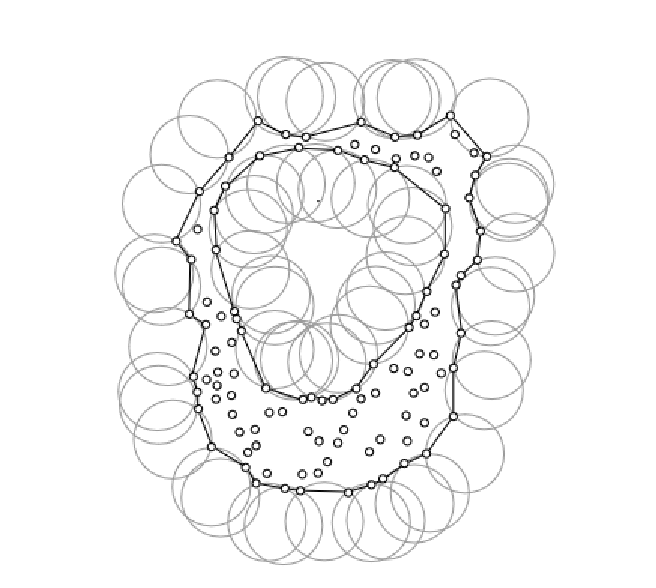
\includegraphics[width=1\linewidth]{97_graphics/related_work/alpha_shapes.pdf}
    \caption{Alpha Shapes Surface Reconstruction Method \parencite{alpha_shapes_stanford} }
    \label{fig:related_work-alpha_shapes}
    \end{minipage}
    \hfill
    \begin{minipage}[b]{0.45\textwidth}
    \centering
    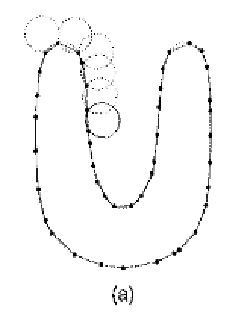
\includegraphics[width=1\linewidth]{97_graphics/related_work/ball_pivoting.pdf}
    \caption{Ball Pivoting Algorithm \parencite{bernardini1999ball}}
    \label{fig:related_work-ball_piv_3}
    \end{minipage}
\end{figure}


\subsection{Ball Pivoting}
Triangle mesh is constructed using the Ball Pivoting algorithm from a set of points \parencite{bernardini1999ball}. The idea behind the ball algorithm is straightforward. Starting from a single edge of the points in the unstructured points, a ball of a specified radius is moved or pivoted without leaving contact with the edge. A single triangle is formed if the ball touches three points, without considering any other points and without falling through. This process is carried on until all reachable edges have been tried. This process can also be viewed in figure \ref{fig:related_work-ball_piv_3}. Ball size can be varied to handle the varying point densities. For example, a larger-sized ball can be used to handle points that are very sparse.

\subsection{Poisson Surface Reconstruction}
By solving a regularized optimization problem, the Poisson surface regeneration approach produces a smooth surface \parencite{kazhdan2006poisson}. Because of this, this method for surface regeneration can be superior to the previously discussed techniques, which results in non-smooth outcomes because the points of the raw point cloud are also the location of the vertex of the final triangle mesh without any change. 

\begin{figure}[htbp]
    \centering
    \begin{minipage}[b]{0.45\textwidth}
    \centering
    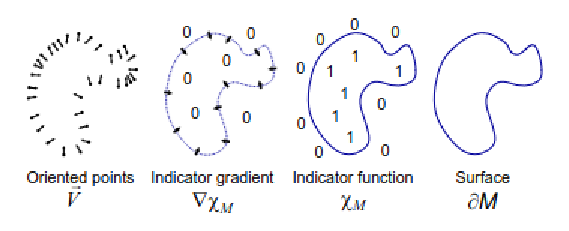
\includegraphics[width=1\linewidth]{97_graphics/related_work/poisson_reconstruction_2.pdf}
    \caption{Poisson reconstruction illustrated in 2D \parencite{kazhdan2006poisson}.}
    \label{fig:related_work-poiss_rec_2}
    \end{minipage}
    \hfill
    \begin{minipage}[b]{0.45\textwidth}
    \centering
    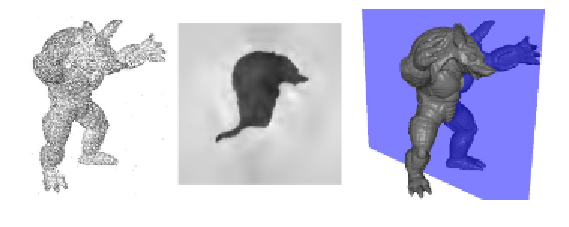
\includegraphics[width=1\linewidth]{97_graphics/related_work/poisson_reconstruction_1.pdf}
    \caption{Poisson Reconstruction illustration.\parencite{kazhdan2006poisson}}
    \label{fig:related_work-poiss_rec_1}
    \end{minipage}
\end{figure}

A model's indicator function and the oriented points, as shown in figure \ref{fig:related_work-poiss_rec_2}, that are collected from its surface are inextricably linked. In particular, the slope of the indicator function is a vector field that is equivalent to the inner surface normal nearly throughout (because the indicator function remains unchanged in almost every place), except in places that are close to the surface. Consequently, the directed point specimens can be considered instances regarding the model's indicator function gradient. Additionally, the indication function can be seen along the plane shown in the figure \ref{fig:related_work-poiss_rec_1} rightmost image and can be viewed by the middle image of the same figure in black color. Triangle meshes are constructed even in low-point density locations and also infer the surface in such locations. The density value of each point indicates if the neighborhood of the point is crowded by other points. Maximum tree depth for the octree defines the resolution of the final reconstructed triangle meshes.

\section{Hidden Point Removal Algorithm}
The "Hidden" Point Removal operator \parencite{katz2007}is used to identify the points in a point cloud that are observable when perceived from a specific angle. Even in the absence of recreating a surface or measuring normals, visibility is ascertained.  This operator can be used on point clouds of different sizes, on sparse and thick point clouds, and on views both inside and outside the cloud. This algorithm is helpful for shadow casting, view-dependent reconstruction, and point cloud visualization. No point is genuinely hidden since points cannot obscure each other (unless they happen to fall along the exact same beam from the viewer). It is possible to identify which points are visible once a surface has been rebuilt from the points. This suggests that the cloud of points has information inherent to it that can be used to extract the point's visibility. Using the intrinsic information of points in the point cloud, the visibility of the points is determined without the need for surface reconstruction. For a point cloud with n number of points, the time complexity of the algorithm is \(O(n\log(n))\) \parencite{katz2007}.

For a point cloud with a "P" number of points, to find the points that are visible from a given viewpoint "C", the \acrshort{hpr} operator can be used. This HPR operator consists of two main steps as shown in figure \ref{fig:realted_work-hpr}. First is Spherical Flipping and second is the creation of a convex hull. 

\subsection{Spherical Flipping}
This step is also called inversion of points. The point "P" is in the geometry where the viewpoint is the Origin of the geometry. A function that maps a point \(p_i\) along the direction of the ray from the viewpoint and is declining in \(||\mathbf{p}_i||\) monotonically, results in spherical flipping. It can be given by equation \ref{eq:spherical_flipping}. Where \(\hat{\mathbf{p}}_i \) is the point after spherical flipping of point \(p_i\). \(R\) is the radius of the sphere and \(||\mathbf{p}_i||\) represents euclidean norm or magnitude of vector \(p_i\).

\begin{equation}\label{eq:spherical_flipping}
\hat{\mathbf{p}}_i = f(\mathbf{p}_i) = \mathbf{p}_i + 2(R - ||\mathbf{p}_i||) \frac{\mathbf{p}_i}{||\mathbf{p}_i||}
\end{equation}


\begin{figure}[htbp]
    \centering
    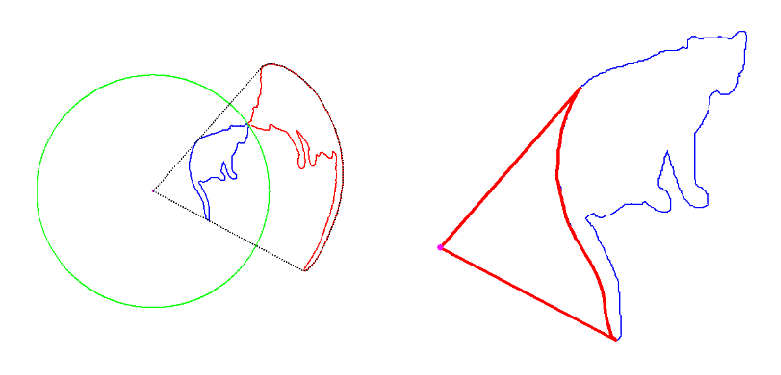
\includegraphics[width=0.5\linewidth]{97_graphics/related_work/spherical_flipping.pdf}
    \caption{Spherical Flipping and Back Projection\parencite{katz2007}}
    \label{fig:related_work-spherical_flipping}
\end{figure}

In the figure \ref{fig:related_work-spherical_flipping}, the green circle represents the Sphere whose center is the viewpoint C or Origin. For a noisy point cloud, the possible alternatives for the radius of the sphere can be found in \parencite{mehra_visibility_XXXX}. Blue curves, internal to the sphere, are projected along the ray from the viewpoint of its image external to the sphere.  This is represented by the red curve on the left side image of figure \ref{fig:related_work-spherical_flipping}. The right image of the figure represents the back project of the convex hull by the red-colored curve.

\begin{figure}[htb]
    \centering
    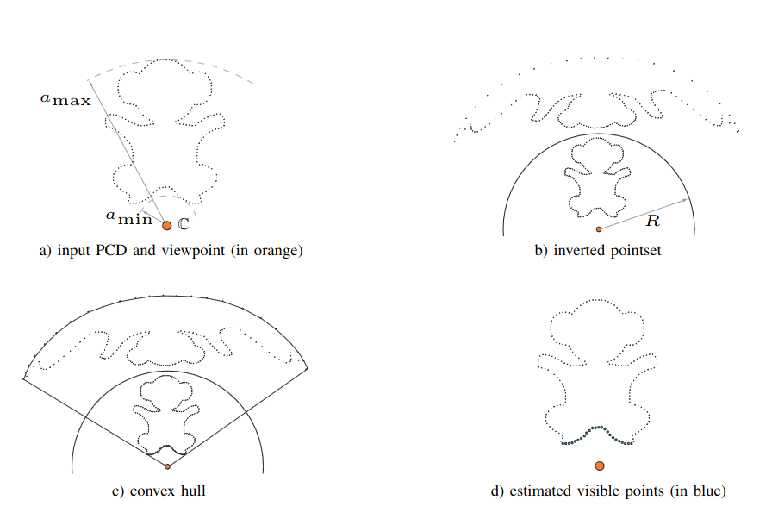
\includegraphics[width=0.8\linewidth]{97_graphics/related_work/hpr_2.pdf}
    \caption{Steps in HPR Algorithm \parencite{mehra_visibility_XXXX}}
    \label{fig:realted_work-hpr}
\end{figure}

\subsection{Calculation of Convex Hull}
In the next step of \acrshort{hpr}, the convex hull of the transformed point \(\hat{\mathbf{p}}_i \) is calculated. The transformed point cloud and the center of viewpoint are used to calculate the convex hull. Visibility of the point \(\hat{\mathbf{p}}_i \) is determined using the location of points respective to the convex hull. According to the algorithm, all the points are visible if the transformed points are located on the convex hull. Selection of the viewpoint C is crucial in the creation of a convex hull because, when C is external to P, points on the object's back may otherwise sit on the convex hull. The two steps can also be viewed in figure \ref{fig:realted_work-hpr}.

\section{Performance Metrices}
\subsection{Confusion Matrix}
The confusion matrix is the foundation of quality assessment matrices. It is a table that combines the test datasets' actual and anticipated values. Confusion matrices are typically employed for classification models and are used to determine the accuracy and correctness of the model. The projected classifications are in rows, and the actual ones are in columns. It is possible to switch the order of the anticipated and actual columns. In the figure, the positive class refers to the "YES" category, and the negative class refers to the "NO" category.

\begin{figure}[htbp]
    \centering
    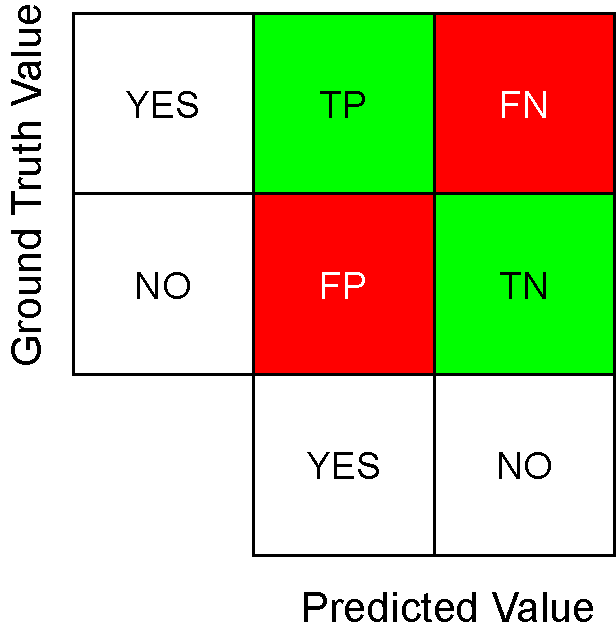
\includegraphics[width=0.5\linewidth]{97_graphics//related_work/conf_matrix.pdf}
    \caption{Confusion Matrix}
    \label{fig:related_work-conf_matrix}
\end{figure}

\begin{itemize}
    \item \textbf{\acrfull{tp} : } If the predicted positive value is the correct classification, these are TP.
    \item \textbf{\acrfull{tn} : }  If the predicted negative value is the correct classification, these are TN.
    \item \textbf{\acrfull{fp} / Type I Error : } For any classification task, if the positive class was predicted which is the incorrect classification. These are FP.
    \item \textbf{\acrfull{fn} / Type II Error : } For any classification task, if the negative class was predicted which is incorrect classification. These are FN.
    \item \textbf{Accuracy : } Tells about the percentage of correct predictions made by the model. Accuracy can be utilized as a benchmark to assess a classification model's performance in a balanced dataset; however, if the dataset is imbalanced (i.e., there is a significant actual difference in the number of positive and negative examples) then choosing a classification model based solely on accuracy is misleading.
    \begin{equation} \label{eq:accuracy}
        Accuracy = \frac{\sum TP + \sum TN}{\sum TP + \sum TN + \sum FP + \sum FN}
    \end{equation}
    \item \textbf{Precision}: The precision of a classifying model indicates the fraction of positively anticipated data that it could correctly identify as positive. Positive Predicted Rate is another name for it.
    \begin{equation}\label{eq:precision}
        \text{Precision} = \frac{\sum TP}{\sum TP + \sum FP}
    \end{equation}
    
    \item \textbf{Recall}: It provides us with the percentage of real positive cases that our algorithm was able to accurately anticipate. True Positive Rate or sensitivity are other terms for recall. A higher recall score indicates that our algorithm can accurately anticipate the majority of positive classes. A lower recall score indicates an inability of our model to accurately forecast the real positive examples.
    \begin{equation}\label{eq:recall}
        \text{Recall} = \frac{\sum TP}{\sum TP + \sum FN}
    \end{equation}
    
    \item \textbf{F1 Score}: A model's accuracy can be determined by calculating the F1-score, which takes into account both the precision and recall of the model's predictions. When working with unbalanced datasets or when the costs associated with false positives and false negatives differ, it is especially helpful. It is the harmonic mean calculated between precision and recall. The best case value of f1-score is 1 and the worst case value is 0. Optimizing recall and precision at the same time increases the value of the f1-score.
    \begin{equation}\label{eq:f1-score}
        \text{F1 Score} = 2 \times \frac{\text{Precision} \times \text{Recall}}{\text{Precision} + \text{Recall}}
    \end{equation}
\end{itemize}


Let's discuss the concept of performance metrics with an example. Consider a HAD system that needs to detect between a person and not a person. Out of 100 observations, 97 observations do not contain a person, and the remaining 3 observations contain a person. If predicting a person is a positive class and predicting a non-person is a negative class, then the metrics can be evaluated. If the HAD system predicted all the 100 observations as non-person then we have \(TP = 0\), \(TN = 97\), \(FP = 0\), and \(FN = 3\). We get an \(Accuracy = 97\%\). Because the dataset is unbalanced, as the number of positive and negative classes is not comparable, considering Accuracy as the determining factor is misleading. So options like F1-Score, Precision, and Recall should be further analysed.

\subsection{Intersection over Union}
\acrfull{iou}, also known as the Jaccard Index, is used to compare how similar two irregular shapes are to one another. It is a performance metric that is used to assess how well object detection algorithms perform, especially when it comes to computer vision and machine learning applications. By assessing the regions of overlap between the anticipated and ground truth bounding boxes, an object detection algorithm's accuracy can be determined. It can be calculated using the equation \ref{eq:iou}. IoU is also utilized in \acrfull{nms}. It is a post-processing method for object detection that helps to choose the most pertinent detected items by removing duplicate detections. A predicted bounding box with a higher IoU has maximum confidence in detecting the object and based on thresholding the IoU value, suitable predictions are finalized.

\begin{equation}\label{eq:iou}
    IoU = \frac{\text{Region of Intersection}}{\text{Region of Union}}
\end{equation}

\begin{figure}[htb]
    \centering
    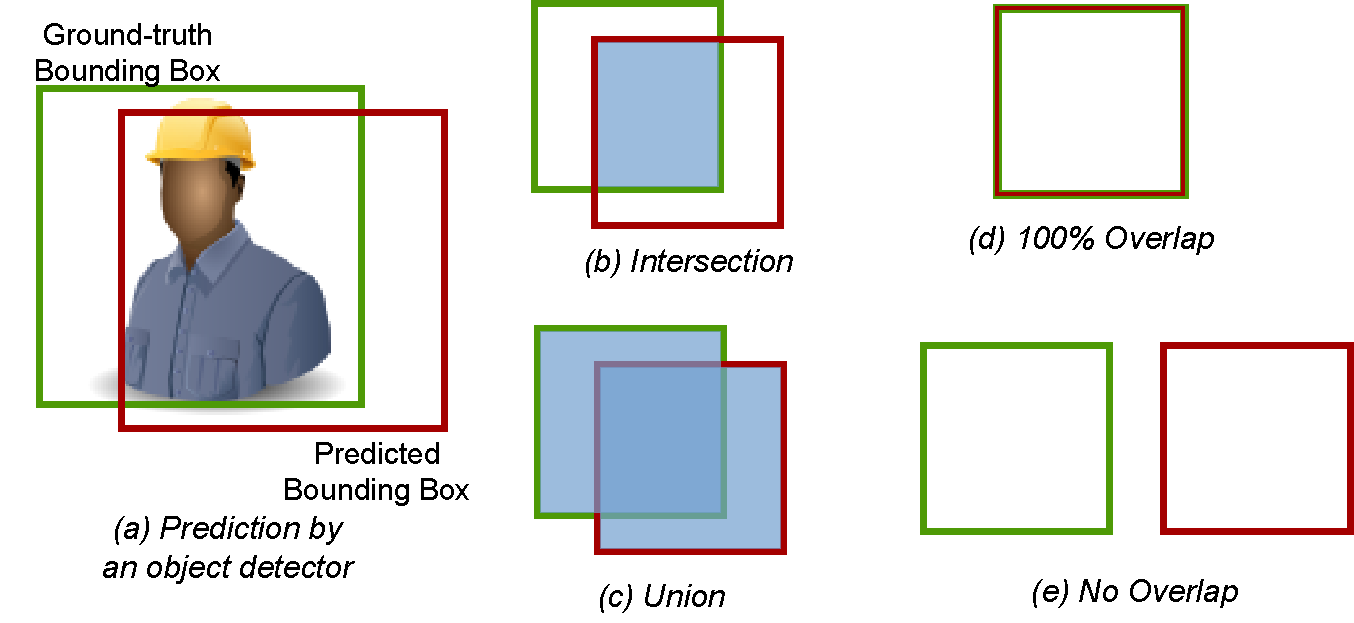
\includegraphics[width=1\linewidth]{97_graphics//related_work/iou.pdf}
    \caption{Intersection over Union}
    \label{fig:related_work-iou}
\end{figure}

Example image (a) in figure \ref{fig:related_work-iou} shows the result of an object detection algorithm. The green colored box is the ground truth and the red colored box is the prediction by the algorithm. By calculating the area of intersection and area of union between the two boxes, IoU can be calculated. Image (d) represents completely overlapped bounding boxes. The IoU in such a case is 1. In case of no overlap between the two regions  (image (e)), the IoU is 0. It is necessary to select an accuracy threshold when utilizing IoU as an evaluation metric. Based on the threshold, the result from an algorithm can be either accepted or rejected.
